\documentclass[10pt]{article}
\usepackage[utf8]{inputenc}
\usepackage[T1]{fontenc}
\usepackage{amsmath}
\usepackage{amsfonts}
\usepackage{amssymb}
\usepackage[version=4]{mhchem}
\usepackage{stmaryrd}
\usepackage{graphicx}
\usepackage[export]{adjustbox}
\graphicspath{ {./images/} }

\title{DIPARTIMENTO DI FISICA E ASTRONOMIA “ETTORE MAJORANA" }

\author{}
\date{}


\begin{document}
\maketitle
\section{A.A. 2022-2023 - FISICA GENERALE I}
\section{PROVA IN ITINERE DEL XXXXXX}
COGNOME

NOME

MATR.

\begin{enumerate}
  \item Due corpi puntiformi \(\mathrm{m}_{1}=100 \mathrm{~g}\) e \(\mathrm{m}_{2}=700 \mathrm{~g}\) sono fissati agli estremi di un'asta rigida di lunghezza 1 \(=48 \mathrm{~cm}\) e di massa trascurabile. La distanza del centro di massa del sistema da \(\mathrm{m}_{1}\) è:
A) \(42 \mathrm{~cm}\)
B) \(24 \mathrm{~cm}\)
C) \(6 \mathrm{~cm}\)
D) \(12 \mathrm{~cm}\)
E) nessuna delle precedenti risposte

  \item Due punti materiali di peso \(\mathrm{p}_{1}=4.3 \mathrm{~N}\) e \(\mathrm{p}_{2}=2.7 \mathrm{~N}\) si muovono di moto rettilineo uniforme con velocità, di verso opposto, \(\mathrm{v}_{1}=4 \mathrm{~m} / \mathrm{s}\) e \(\mathrm{v}_{2}=-7 \mathrm{~m} / \mathrm{s}\). Calcolare la velocità del centro di massa.
A) \(2.42 \mathrm{~m} / \mathrm{s}\)
B) \(-0.24 \mathrm{~m} / \mathrm{s}\)
C) \(6.25 \mathrm{~m} / \mathrm{s}\)
D) zero
E) nessuna delle precedenti risposte

  \item Un cannone, di massa \(\mathrm{M}=2500 \mathrm{~kg}\) e inizialmente fermo, spara un proiettile di massa \(\mathrm{m}=5 \mathrm{~kg}\) con velocità \(\mathrm{v}=300 \mathrm{~m} / \mathrm{s}\). Calcolare l'energia cinetica del cannone subito dopo lo sparo.
A) \(112.5 \mathrm{MJ}\)
B) \(225000 \mathrm{~J}\)
C) \(450 \mathrm{~J}\)
D) dati non sufficienti
E) nessuna delle precedenti risposte

  \item Una palla da baseball di 150 g lanciata alla velocità di \(41.6 \mathrm{~m} / \mathrm{s}\) viene respinta indietro al lanciatore con la velocità di \(61.5 \mathrm{~m} / \mathrm{s}\). La mazza resta in contatto con la palla per \(4.70 \mathrm{~ms}\). Qual è la forza media esercitata dalla mazza sulla palla?
A) \(5340 \mathrm{~N}\)
B) \(3290 \mathrm{~N}\)
C) \(787.5 \mathrm{~N}\)
D) forza nulla
E) nessuna delle precedenti risposte

  \item Un corpo rigido di massa \(m=4 \mathrm{~kg}\), può ruotare attorno ad un asse passante per un suo punto.

\end{enumerate}

Determinare il momento di inerzia I rispetto all'asse di rotazione, sapendo che quello rispetto all'asse parallelo passante per il centro di massa e distante \(0.3 \mathrm{~m}\) dal primo è \(\mathrm{I}_{\mathrm{cm}}=0,12 \mathrm{~kg} \mathrm{~m}\).
A) \(0.36 \mathrm{~kg} \mathrm{~m}^{2}\)
B) \(0.12 \mathrm{~kg} \mathrm{~m}^{2}\)
C) \(0.48 \mathrm{~kg} \mathrm{~m}^{2}\)
D) \(15 \mathrm{~kg} \mathrm{~m}^{2}\)
E) nessuna di queste risposte

\begin{enumerate}
  \setcounter{enumi}{5}
  \item Una ruota (anello sottile \(\mathrm{I}=\mathrm{mR}^{2}\) ) di massa \(31.4 \mathrm{~kg}\) e raggio \(1.21 \mathrm{~m}\) ruota alla velocità angolare di 283 giri/min attorno al suo asse. Trovare la potenza media richiesta per fermarla in \(14.8 \mathrm{~s}\).
A) \(88 \mathrm{~W}\)
B) \(136 \mathrm{~W}\)
C) \(1360 \mathrm{~W}\)
D) \(12.5 \mathrm{~W}\)
E) nessuna di queste possibilità 7. Due corpi puntiformi di massa uguale sono fissati agli estremi di un'asta rigida orizzontale di lunghezza \(50 \mathrm{~cm}\) e di massa trascurabile, posta in rotazione con velocità angolare di \(15 \mathrm{rad} / \mathrm{s}\) attorno ad un asse verticale passante per il centro di massa del sistema. Ad un certo istante, mediante un meccanismo interno, l'asta si allunga allontanando ciascuna massa di \(5 \mathrm{~cm}\) dall'asse di rotazione. Calcolare la nuova velocità angolare.
A) \(10.4 \mathrm{rad} / \mathrm{s}\)
B) \(15 \mathrm{rad} / \mathrm{s}\)
C) \(18.5 \mathrm{rad} / \mathrm{sec}\)
D) l'asta si ferma
E) nessuna delle precedenti risposte

  \item Un cilindro \(\left(\mathrm{I}_{\mathrm{c}}=1 / 2 \mathrm{~m} \mathrm{R}^{2}\right)\), inizialmente fermo, scende senza strisciare lungo un piano inclinato. La velocità del suo centro di massa alla base del piano inclinato è di \(2 \mathrm{~m} / \mathrm{s}\). Determinare l'altezza h di partenza.
A) dati non sufficienti
B) \(30.6 \mathrm{~cm}\)
C) \(20.4 \mathrm{~cm}\)
D) \(41.3 \mathrm{~cm}\)
E) nessuna delle precedenti risposte

  \item Due corpi \(\mathrm{m}_{1}=0.2 \mathrm{~kg}\) e \(\mathrm{m}_{2}=0.3 \mathrm{~kg}\) si muovono lungo la stessa direzione e lo stesso verso con velocità \(\mathrm{v}_{1}\) \(=3 \mathrm{~m} / \mathrm{s}\) e \(\mathrm{v}_{2}=2 \mathrm{~m} / \mathrm{s}\). Determinare la variazione di energia cinetica del sistema in seguito ad un urto completamente anelastico.
A) \(-0.06 \mathrm{~J}\)
B) - \(3.2 \mathrm{~J}\)
C) \(+3.2 \mathrm{~J}\)
D) zero
E) nessuna di tali risposte è corretta

  \item Due masse \(m_{1}=200\) g e \(m_{2}=400 \mathrm{~g}\) sono fissate agli estremi di una fune inestensibile e di massa trascurabile messa a cavallo di una puleggia di massa \(\mathrm{M}\) e raggio \(\mathrm{R}=10 \mathrm{~cm}\), libera di ruotare senza attrito attorno ad un asse passante per il suo centro. Sapendo che le masse sono soggette ad una accelerazione pari a \(1 \mathrm{~m} / \mathrm{s}^{2}\), calcolare il momento d'inerzia della puleggia rispetto al suo asse. Si supponga che la fune non scivoli sulla puleggia.
A) zero
B) \(0.2610^{-2} \mathrm{~kg} \mathrm{~m}^{2}\)
C) \(1.3610^{-2} \mathrm{~kg} \mathrm{~m}^{2}\)
D) \(2.610^{-2} \mathrm{~kg} \mathrm{~m}^{2}\)
E) nessuna delle precedenti risposte

\end{enumerate}

\begin{center}
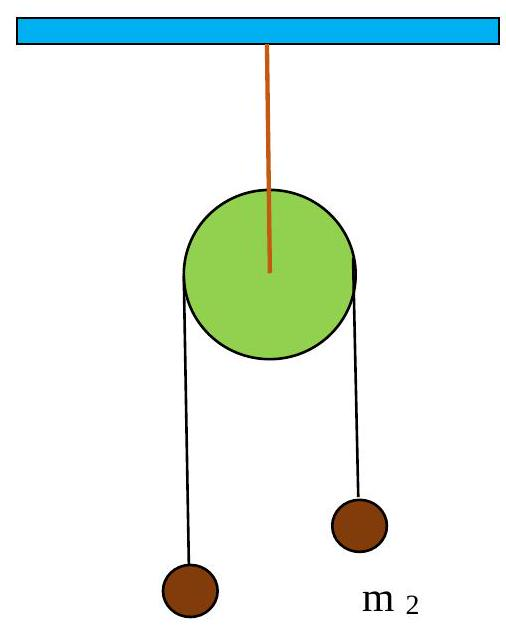
\includegraphics[max width=\textwidth]{2023_05_14_22be0453ff08c016e50dg-2}
\end{center}

\(\mathrm{m}_{1}\)


\end{document}